\documentclass[a4paper,12pt]{article}

\usepackage{mystyle}
\usepackage{gensymb}

\graphicspath{ {images/} }

\definecolor{my-red}{RGB}{176, 0, 0}
\definecolor{my-blue}{RGB}{0, 0, 153}


\author{Алексеев Василий}


\title{Семинар 10}
\date{17 ноября + 23 ноября 2020}


\begin{document}
  \maketitle
  
  \tableofcontents

  \thispagestyle{empty}
  
  \newpage
  
  \pagenumbering{arabic}


  \section{Аффинные преобразования плоскости}
  
  \subsection{Про отображения}
  
  Отображение $f$ из $\mathcal X$ в $\mathcal Y$~---~это закон, по которому элементу $x \hm\in \mathcal X$ ставится в соответствие элемент $y \hm\in \mathcal Y$.
  Область определения функции $f$~---~это подмножество элементов $D_f \hm\subseteq \mathcal X$, на которых функция определена\footnote{$D_f$~---~одно из возможных обозначений обозначения области определения, есть и другие}.
  Область значений функции $f$~---~это образ области значений $D_f$, то есть $\{y \hm\in \mathcal Y \hm\mid \exists x \hm\in \mathcal X\colon f(x) \hm= y\}$.
  
  Дадим ещё пару определений, касающихся свойств отображений.
  
  \begin{definition}[Инъекция]
    Функция \emph{инъективна}, если разные элементы $\mathcal X$ под действием функции $f$ переводятся в разные элементы $\mathcal Y$:
    \[
      x_1, x_2 \in \mathcal X,\ x_1 \not= x_2 \Rightarrow f(x_1) \not= f(x_2)
    \]
  \end{definition}
  
  \begin{definition}[Сюръекция]
    Функция \emph{сюръективна}, если для любого элемента из $\mathcal Y$ существует прообраз:
    \[
      \forall y \in \mathcal Y \exists x \in \mathcal X\colon f(x) = y
    \]
  \end{definition}
  
  \begin{definition}[Биекция]
    Функция \emph{биективна}, если для любого элемента из $\mathcal Y$ существует единственный прообраз, то есть если функция инъективна и сюръективна.
  \end{definition}
  
  \begin{definition}[Композиция отображений]
    Пусть есть отображения $f\colon \mathcal X \hm\to \mathcal Y$ и $g\colon \mathcal Y \hm\to \mathcal Z$, причём $f(X) \hm\subseteq D_g \hm\subseteq Y$.
    Тогда композицией\footnote{Автор конспекта не смог выяснить, является ли порядок слов важным при обозначении композиции или нет. Например, одно ли то же ``композиция $f$ и $g$'' и ``композиция $g$ и $f$''? Кажется, в русском языке на словах порядок отображений в композиции не выражается, только в виде формулы...} отображений $f$ и $g$ называется отображение $h\colon \mathcal X \hm\to \mathcal Z$, такое что
    \[
      h(x) = g(f(x))
    \]
    
    Отображение $h$ может обозначаться как $g\circ f$ или $gf$.
  \end{definition}

  \begin{theorem}
    Любая функция $f\colon \mathcal X \hm\to \mathcal Y$ может быть представлена как композиция сюръекции, биекции и инъекции (\ref{fig:tribute-to-algebraic}).
  \end{theorem}
  
  \begin{proof}
    \begin{figure}
      \centering
      
      \includegraphics[width=0.8\columnwidth]{tribute-to-algebraic-approach}
      
      \caption{Любое отображение $f$ можно представить как композицию отображений.}
      \label{fig:tribute-to-algebraic}
    \end{figure}
    
    Пусть $\alpha\colon \mathcal X \hm\to \mathcal X_f$~---~функция, которая каждый элемент $x \hm\in \mathcal X$ переводит в подмножество элементов $S(x) \hm\subseteq \mathcal X$, такое что $\forall x' \hm\in \mathcal X\colon f(x') \hm= f(x) \hm\Rightarrow x' \hm\in S(x)$.
    А $X_f$~---~множество таких подмножеств из $\mathcal X$, на которых значение функции $f$ одинаково.
    Очевидно, отображение $\alpha$ сюръективно.
    
    Пусть $\beta\colon \mathcal X_f \hm\to f(\mathcal X)$~---~отображение, которое каждый элемент $S \hm\in \mathcal X_f$ переводит в значение функции $f$ на элементе $x \hm\in S$.
    По построению $\mathcal X_f$, не важно, какой элемент выбрать из $S$ для вычисления значения функции $f$.
    Очевидно, отображение $\beta$ биективно.
    
    Пусть $\gamma\colon f(\mathcal X) \hm\to \mathcal Y$~---~тождественное отображение, то есть $\gamma(y) \hm= y$, $\forall y \hm\in f(\mathcal X)$.
    Очевидно, $\gamma$~---~инъективное отображение.
    
    Таким образом, $f \hm= \gamma \circ \beta \circ \alpha$.
  \end{proof}
  
  Рассмотрим небольшую задачу на абстрактные свойства отображений.
  
  \subsection{\# 12.1(2, 4)}
  
  Для отображения $f\colon \mathcal X \to \mathcal Y$ доказать, что
  
  \begin{enumerate}
    \setcounter{enumi}{1}
    
    \item $f(A_1 \cup A_2) = f(A_1) \cup f(A_2)$
    
    \setcounter{enumi}{3}
    
    \item $f(A_1 \cap A_2) \subseteq f(A_1) \cap f(A_2)$
  \end{enumerate}
  
  \begin{solution}
    Начнём с первого пункта.
    Чтобы доказать требуемое, достаточно показать, что произвольная точка из $f(A_1 \cup A_2)$ лежит также и в $f(A_1) \cup f(A_2)$ и наоборот, что произвольная точка из $f(A_1) \cup f(A_2)$ лежит также и в $f(A_1 \cup A_2)$.
    
    Пусть $y \hm\in f(A_1 \cup A_2)$.
    Это значит, что $\exists x \hm\in A_1 \hm\cup A_2\colon f(x) \hm= y$.
    Если $x \hm\in A_1$, то $f(x) \hm\in f(A_1)$, если же $x \hm\in A_2$, то $f(x) \hm\in f(A_2)$.
    В любом случае $f(x) \hm\in f(A_1) \hm\cup f(A_2)$.
    
    Пусть теперь $y \hm\in f(A_1) \hm\cup f(A_2)$.
    Это значит, что $\exists x \hm\in A_1\colon f(x) \hm= y$ или $\exists x \hm\in A_2\colon f(x) \hm= y$.
    Но это можно переписать как $\exists x \hm\in A_1 \hm\cup A_2\colon f(x) \hm= y$, а это и значит, что $f(x) \hm\in f(A_1 \cup A_2)$.
    
    \bigskip
    
    Теперь докажем второй пункт.
    Пусть $y \hm\in f(A_1 \cap A_2)$.
    Это значит, что $\exists x \hm\in A_1 \hm\cap A_2\colon f(x) \hm= y$.
    Из того, что $x \hm\in A_1$, следует, что $f(x) \hm\in f(A_1)$.
    Аналогично, $x \hm\in A_2 \hm\Rightarrow f(x) \hm\in f(A_2)$.
    В итоге $f(x) \hm\in f(A_1) \hm\cap f(A_2)$.
    
    Покажем, что второе включение не выполняется, то есть что может $\exists y \hm\in f(A_1) \hm\cap f(A_2)$, такой что $y \hm{\not\in} f(A_1 \cap A_2)$.

    \begin{figure}
      \centering
      
      \includegraphics[width=0.8\columnwidth]{cap-not-cap}
      
      \caption{$A_1, A_2$ и $f$, такие что $f(A_1) \hm\cap f(A_2) \hm{\not=} \noth$, но $A_1 \hm\cap A_2 \hm= \noth$.}
      \label{fig:cap-not-cap}
    \end{figure}

    Выберем $A_1$ и $A_2$ так, чтобы $f(A_1) \hm\cap f(A_2) \hm{\not=} \noth$ (отображение $f$, хоть и ``дано в условии'', произвольное, и его тоже можно подбирать) и $A_1 \hm\cap A_2 \hm= \noth$ (\ref{fig:cap-not-cap}).
    И получаем, что $\bigl(f(A_1) \hm\cap f(A_2)\bigr) \hm\cap f(A_1 \cap A_2) \hm= \noth$.
  \end{solution}
  
  
  \subsection{Про линейные и аффинные преобразования}
  
  Перейдём к случаю отображений из одной плоскости в другую $f\colon P \hm\to Q$.
  Даже в более частному случаю отображений из плоскости в ту же плоскость $f\colon P \hm\to P$, которые ещё называют \emph{преобразованиями}.
  
  Примерами преобразований плоскости могут служить поворот, параллельный перенос, симметрия относительно оси или точки, гомотетия\footnote{Гомотетия с центром в точке $O$ и коэффициентом $k \not=0 $ каждой точке $M$ ставит в соответствие точку $M^\star$, так что $\vv{OM^\star} \hm= k\vv{OM}$}.
  % TODO: pic
  
  Преобразования плоскости тоже могут быть инъективными, сюръективными, биективными.
  Например, отображение всех точек плоскости в одну и ту же точку не является ни инъективным, ни сюръективным отображением.
  Можно привести пример инъективного отображения плоскости в круг\footnote{
    Например, круг с центром в начале координат.
    Каждую точку $M$ плоскости можно взаимно однозначно перевести в точку круга: через $M$ и начало координат можно провести прямую $l$ и рассмотреть часть этой прямой внутри круга (отрезок).
    Известно, что отрезок равносилен всей числовой прямой, поэтому между отрезком и прямой $l$ можно установить взаимно однозначное соответствие, и точка $M$ при этом перейдёт в какую-то точку отрезка.
  }.
  В качестве сюръективного отображения можно, например, в некоторой декартовой системе координат на плоскости взять отображение
  \[
    (x, y) \mapsto \left(x^2 - y^2, 2xy\right)
  \]
  
  В последнем примере мы обратились к координатной записи преобразования.
  Преобразование (и вообще отображение) переводит точку в точку.
  Поэтому, выбрав систему координат на плоскости, закон сопоставления точек можно выразить через их координаты, указав, как вычислять $x$ и $y$ образа.
  
  \begin{definition}
    \emph{Линейным} называется преобразование, которое в некоторой декартовой системе координат можно выразить формулами
    \begin{equation}
      \label{eq:linear}
      \left\{
        \begin{aligned}
          &x^\star = a_1 x + b_1 y + c_1\\
          &y^\star = a_2 x + b_2 y + c_2
        \end{aligned}
      \right.
    \end{equation}
    
    При этом $a_i, b_i, c_i \hm\in \RR,\ i = 1, 2$.
  \end{definition}
  
  Линейное преобразование плоскости $f$ порождает следующее преобразование векторов:
  \[
    \vv{AB} \overset{f}{\mapsto} \vv{f(A)f(B)}
  \]
  Преобразование векторов можно обозначать той же буквой, что и преобразование координат (потому что по смыслу и так понятно, о каком преобразовании идёт речь).
  Координатная запись преобразования вектора $\bds v \hm= (\alpha, \beta)$:
  \begin{equation}
    \left\{
      \begin{aligned}
          &\alpha^\star = a_1 \alpha + b_1 \beta\\
          &\beta^\star = a_2 \alpha + b_2 \beta
      \end{aligned}
    \right.
  \end{equation}
  
  Откуда следуют свойства:
  \[
    \left\{
      \begin{aligned}
        &f(\bds v + \bds u) = f(\bds v) + f(\bds u)\\
        &f(\lambda \bds v) = \lambda f(\bds v),\quad \lambda \in \RR
      \end{aligned}
    \right.
  \]
  
  В качестве линейного преобразования можно привести, например, преобразование поворота
  \[
    \left\{
      \begin{aligned}
        &x^\star = x\cos\phi - y\sin\phi\\
        &y^\star = x\sin\phi + y\cos\phi
      \end{aligned}
    \right.
  \]
  является линейным.
  
  И то преобразование, переводящее плоскость в одну точку (например в ноль)
  \[
    \left\{
      \begin{aligned}
        &x^\star = 0\\
        &y^\star = 0
      \end{aligned}
    \right.
  \]
  тоже будет линейным, но...
  
  \begin{definition}
    \emph{Аффинным} называется взаимно однозначное (биективное) преобразование плоскости.
  \end{definition}
  
  Поворот будет аффинным преобразованием, а отображение в одну точку~---~уже не будет аффинным.
  \emph{Критерием аффинности} преобразования~---~чтобы решение системы (\ref{eq:linear}) всегда существовало и было единственно~---~является отличие от нуля определителя системы (\ref{eq:linear}):
  \[
    \begin{vmatrix} a_1 & b_1\\ a_2 & b_2\end{vmatrix} \not= 0
  \]
  
  % TODO: про неподвижную точку, инвариантное мнодествуо?
  
  
  \subsubsection{Некоторые свойства аффинных преобразований}
  
  Под действием аффинного преобразования $f$
  \begin{enumerate}
    \item[1)] прямая переходит в прямую:
    \[
        \left\{
          \begin{aligned}
            &\vv{OM} = \bds r_0 + \bds a t\\
            &\vv{OM^*} = \vv{OO^*} + \vv{O^*M^*}
          \end{aligned}
        \right.
        \Rightarrow
        \vv{OM^*} = \vv{OO^*} + f(\vv{OM}) = \bigl(\vv{OO^*} + f(\bds r_0)\bigr) + f(\bds a) t
    \]
    \item[2)] отрезок переходит в отрезок: как я прямой, только $t$~---~не произвольное $\RR$ число, а из некоторого отрезка $[a, b]$;
    \item[3)] параллельные прямые переходят в параллельные прямые: если образы не параллельны, то они пересекаются~---~значит, есть общая точка, у которой два различных прообраза (по одному на каждой из исходных параллельных прямых)~---~противоречие с взаимной однозначностью преобразования;
    \item[4)] кривая второго порядка переходит в кривую второго порядка;
    \item[5)] ...при этом сохраняется класс кривой (эллипс, гипербола, парабола, точка, прямая, пара пересекающихся прямых, пара параллельных прямых);
    \item[6)] ...более того, для любых двух кривых второго порядка одного класса существует аффинное преобразование, которое переводит одну кривую в другую.
  \end{enumerate}
  
  
  \section{Задачи}
  
  \subsection{\# 12.42(1)}
  
  Найти все неподвижные точки аффинного преобразования
  \[
    \left\{
      \begin{aligned}
        &x^* = 7x - 3y\\
        &y^* = x + y
      \end{aligned}
    \right.
  \]
  
  \begin{solution}
    Неподвижная точка~---~такая, которая под действием преобразования переходит в себя: $x^* \hm= x$, $y^* \hm= y$, то есть
    \[
      \left\{
        \begin{aligned}
          &x = 7x - 3y\\
          &y = x + y
        \end{aligned}
      \right.
      \Leftrightarrow
      \left\{
        \begin{aligned}
          &6x - 3y = 0\\
          &x = 0
        \end{aligned}
      \right.
      \Leftrightarrow
      (x, y) = (0, 0)
    \]
  \end{solution}
  
  
  \subsection{\# 12.43(1)}
  
  Найти инвариантные прямые линейного преобразования
  \[
    \left\{
      \begin{aligned}
        &x^* = 2x + 3y\\
        &y^* = -y
      \end{aligned}
    \right.
  \]
  
  \begin{solution}
    Инвариантная прямая $l$~---~такая, все точки которой под действием преобразования остаются на той же прямой, то есть $(x, y) \hm\in l \hm\Rightarrow (x^*, y^*) \hm\in l$.
    Будем искать инвариантную прямую в виде $Ax \hm+ By \hm+ C \hm= 0$.
    Тогда точка $(x, y)$, лежащая на прямой, должна удовлетворять системе
    \[
      \left\{
        \begin{aligned}
          &Ax + By + C = 0\\
          &Ax^* + By^* + C = 0
        \end{aligned}
      \right.
      \Leftrightarrow
      \left\{
        \begin{aligned}
          &Ax + By + C = 0\\
          &A\cdot (2x + 3y) + B\cdot (-y) + C = 0
        \end{aligned}
      \right.
      \Leftrightarrow
      \left\{
        \begin{aligned}
          &Ax + By + C = 0\\
          &2Ax + (3A - B)y + C = 0
        \end{aligned}
      \right.
    \]
    
    Системе удовлетворяет любая точка исходной прямой.
    Второе уравнение системы также описывает некоторую прямую.
    Значит, прямые, которые заданы первым и вторым уравнениями системы, должны быть одной и той же прямой:
    \[
      \frac{2A}{A} = \frac{3A - B}{B} = \frac{C}{C}
    \]
    
    Далее надо рассмотреть несколько случаев.
    Например, если $A \hm= 0$, то $\dfrac{-B}{B} \hm= \dfrac{C}{C}$.
    При этом точно $B \hm{\not=} 0$.
    Поэтому получаем $-1 \hm= \dfrac{C}{C}$, что в данной записи означает, что $C \hm= 0$.
    Таким образом, первая инвариантная прямая (в качестве $B$ можно взять единицу):
    \[
      y = 0
    \]
    
    Пусть теперь $A \hm{\not=} 0$.
    Тогда получаем $2 \hm= \dfrac{3A - B}{B} = \dfrac{C}{C}$.
    Снова получаем, что $C \hm= 0$.
    Коэффициент $B$ находим из соотношения $2 \hm= \dfrac{3A - B}{B} \hm{\Leftrightarrow} 3A \hm- B \hm= 2B$.
    Получается, что $B \hm= A$.
    И уравнение инвариантной прямой (при $A \hm= 1$, например):
    \[
      x + y = 0
    \]
    
  \end{solution}
  
  
  \subsection{\# 12.48(1)}
  
  Дано аффинное преобразование
  \[
    \left\{
      \begin{aligned}
        &x^* = 2x + 3y\\
        &y^* = 3x + 5y
      \end{aligned}
    \right.
  \]
  
  Надо составить уравнение образа кривой $x^2 \hm+ y^2 \hm= 1$.
  
  \begin{solution}
    Уравнение образа кривой~---~соотношение между координатами точек, такое что точки образа и только они удовлетворяют этому соотношению.
    Аффинное преобразование взаимно однозначно~---~значит, можно выразить исходные координаты $x, y$ через $x^*, y^*$:
    \[
      \left\{
        \begin{aligned}
          &x = h_1(x^*, y^*) = \ldots = 5x^* - 3y^*\\
          &y = h_2(x^*, y^*) = \ldots = -3x^* + 2y^*
        \end{aligned}
      \right.
    \]
    
    Таким образом, уравнение исходной кривой
    \[
      x^2 + y^2 \hm= 1
    \]
    ``переходит'' в уравнение образа кривой
    \[
      h_1^2(x^*, y^*) + h_2^2(x^*, y^*) \hm= 1
        \Leftrightarrow (5x^* - 3y^*)^2 + (-3x^* + 2y^*)^2 = 1
        \Leftrightarrow {34x^*}^2 - 42xy + {13y^*}^2 - 1 = 0
    \]
  \end{solution}
  
  
  \subsection{\# 12.53(6, 8)}
  
  Вывести формулы, задающие данные преобразования плоскости:
  \begin{enumerate}
    \setcounter{enumi}{5}
    
    \item Симметрия относительно прямой $l\colon 3x + 4y - 1 = 0$
    
    \setcounter{enumi}{7}
    
    \item Сжатие к прямой $m\colon x + y - 2 = 0$ с коэффициентом $1/3$
  \end{enumerate}
  
  \begin{solution}
    \begin{figure}
      \centering
      
      \includegraphics[width=0.5\columnwidth]{simmetria-linea}
      
      \caption{Преобразование симметрии относительно прямой.}
      \label{fig:simmetria-linea}
    \end{figure}
    
    Чтобы получить уравнения, задающие симметрию относительно прямой, рассмотрим произвольную точку плоскости $M(x, y)$ (\ref{fig:simmetria-linea}).
    Образ этой точки~---~точка $M^\star(x^\star, y^\star)$.
    Введём дополнительно точку $M_\perp$~---~ортогональную проекцию точки $M$ на прямую $l$.
    Симметрия относительно прямой~---~такое преобразование, что $\vv{M^\star M} \hm= 2 \vv{M_\perp M}$.
    Выпишем все получившиеся условия, чтобы потом переписать их через координаты точек
    \[
      \left\{
        \begin{aligned}
          &\vv{M_\perp M} \perp l\\
          &M_\perp \in l\\
          &\vv{M^\star M} = 2 \vv{M_\perp M}
        \end{aligned}
      \right.
    \]
    
    Из первых двух уравнений можно найти координаты точки $M_\perp(x_1, y_1)$:
    \[
      \left\{
        \begin{aligned}
          &(x_1 - x_0) \cdot (-4) + (y_1 - y_0) \cdot 3 = 0\\
          &3x_1 + 4y_1 - 1 = 0
        \end{aligned}
      \right.
      \Rightarrow \ldots
      \Rightarrow \left\{
        \begin{aligned}
          &x_1 = \frac{3 + 16x_0 - 12y_0}{25}\\
          &y_1 = \frac{4 - 12x_0 + 9y_0}{25}
        \end{aligned}
      \right.
    \]
    
    И координаты точки-образа можно найти как
    \[
      \left\{
        \begin{aligned}
          &x^\star = x_0 + 2 \cdot (x_1 - x_0)\\
          &y^\star = y_0 + 2 \cdot (y_1 - y_0)
        \end{aligned}
      \right.
    \]
    
    \bigskip
    
    \begin{figure}
      \centering
      
      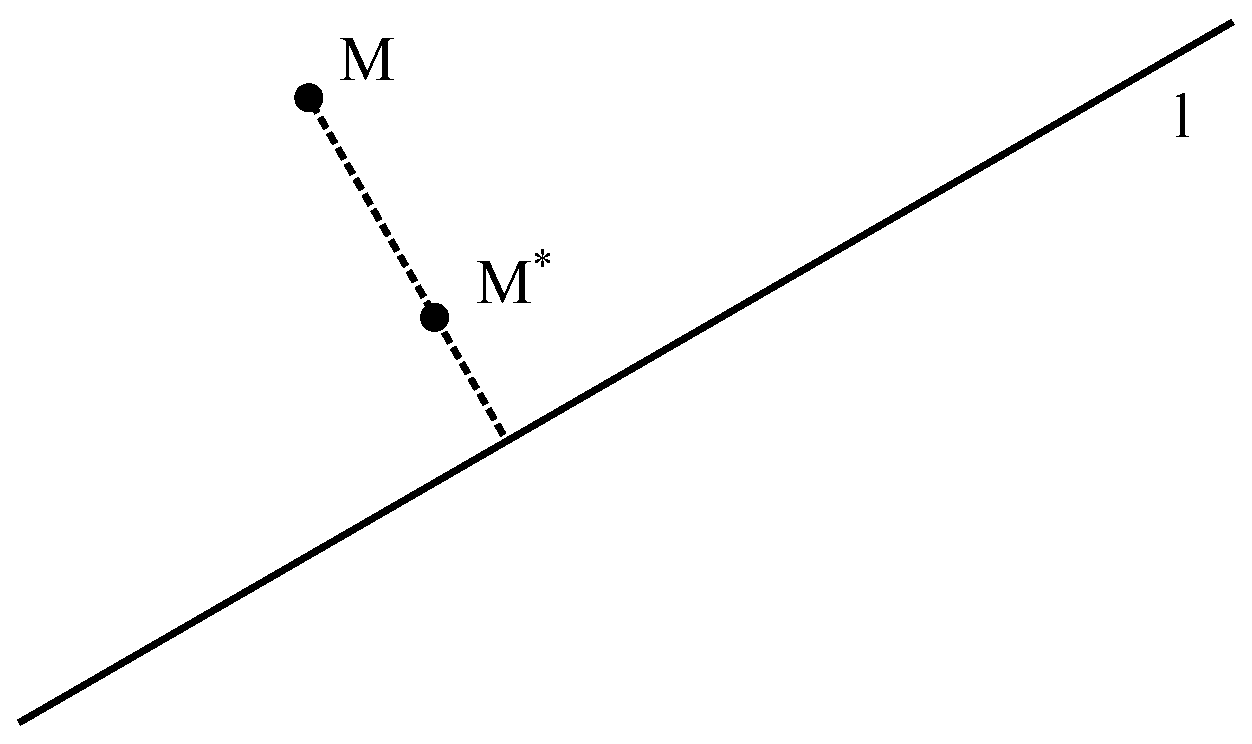
\includegraphics[width=0.5\columnwidth]{compressione-linea}
      
      \caption{Преобразование сжатия к прямой.}
      \label{fig:compressione-linea}
    \end{figure}
    
    Перейдём ко второму пункту задачи (про сжатие к прямой).
    Идея решения точно такая же: рассмотрим точку $M(x, y)$ и её образ $M^\star(x^\star, y^\star)$, получающийся в результате преобразования (\ref{fig:compressione-linea}).
    Суть сжатия к прямой $m$ с коэффициентом $k$ в том, что расстояния от точек до прямой $m$ изменяются в $k$ раз.
    При этом точка-образ лежит $M^\star$ на перпендикуляре из исходной точки к прямой, и по ту же сторону от прямой.
    Выпишем систему из упомянутых условий (то, что точки $M$ и $M^\star$ лежат по одну сторону от прямой, мы используем позднее):
    \[
      \left\{
        \begin{aligned}
          &d(M^\star, m) = \frac{1}{3} \cdot d(M, m)\\
          &\vv{M^\star M} \perp m\\
        \end{aligned}
      \right.
    \]
    
    Расписывая через координаты, получаем
    \[
      \left\{
        \begin{aligned}
          &\frac{|x^\star + y^\star - 2|}{\sqrt{2}} = \frac{1}{3} \cdot \frac{|x + y - 2|}{\sqrt{2}}\\
          &(x^\star - x) \cdot (-1) + (y^\star - y) \cdot 1 = 0\\
        \end{aligned}
      \right.
    \]
    
    Модули в первом уравнении системы раскрываются с одинаковыми знаками (как раз потому, что обе точки лежат по одну сторону от прямой $m$, до которой вычисляется расстояние).
    Решая систему, находим координаты точки-образа через координаты исходной точки, то есть получаем формулы преобразования:
    \[
      \left\{
        \begin{aligned}
          &x^\star = \frac{2}{3}x - \frac{1}{3}y + \frac{2}{3}\\
          &y^\star = -\frac{1}{3}x + \frac{2}{3}y + \frac{2}{3}
        \end{aligned}
      \right.
    \]
  \end{solution}
  
  
  \subsection{\# 9.13(3)}
  
  Определить тип кривой второго порядка
  \[
    (x - y - 3)(x + y + 3) = 4
  \]
  
  \begin{solution}
    Сделаем напрашивающуюся замену:
    \[
      \left\{
        \begin{aligned}
          &x^\star = x - y - 3\\
          &y^\star = x + y + 3
        \end{aligned}
      \right.
    \]
    
    Преобразование, очевидно, линейное.
    Определитель системы отличен от нуля, поэтому преобразование взаимно однозначное (в итоге~---~аффинное).
    А кривая
    \[
      x^\star y^\star = 4
    \]
    очевидно, является гиперболой.
    Так как при аффинном преобразовании тип кривой второго порядка сохраняется, то и исходная система описывает гиперболу.
  \end{solution}
  
  
  \subsection{\# 12.31}
  
  Доказать, что две касательные к эллипсу (или гиперболе) параллельны тогда и только тогда, когда точки касания и центр кривой лежат на одной прямой.
  
  \begin{solution}
    \begin{figure}
      \centering
      
      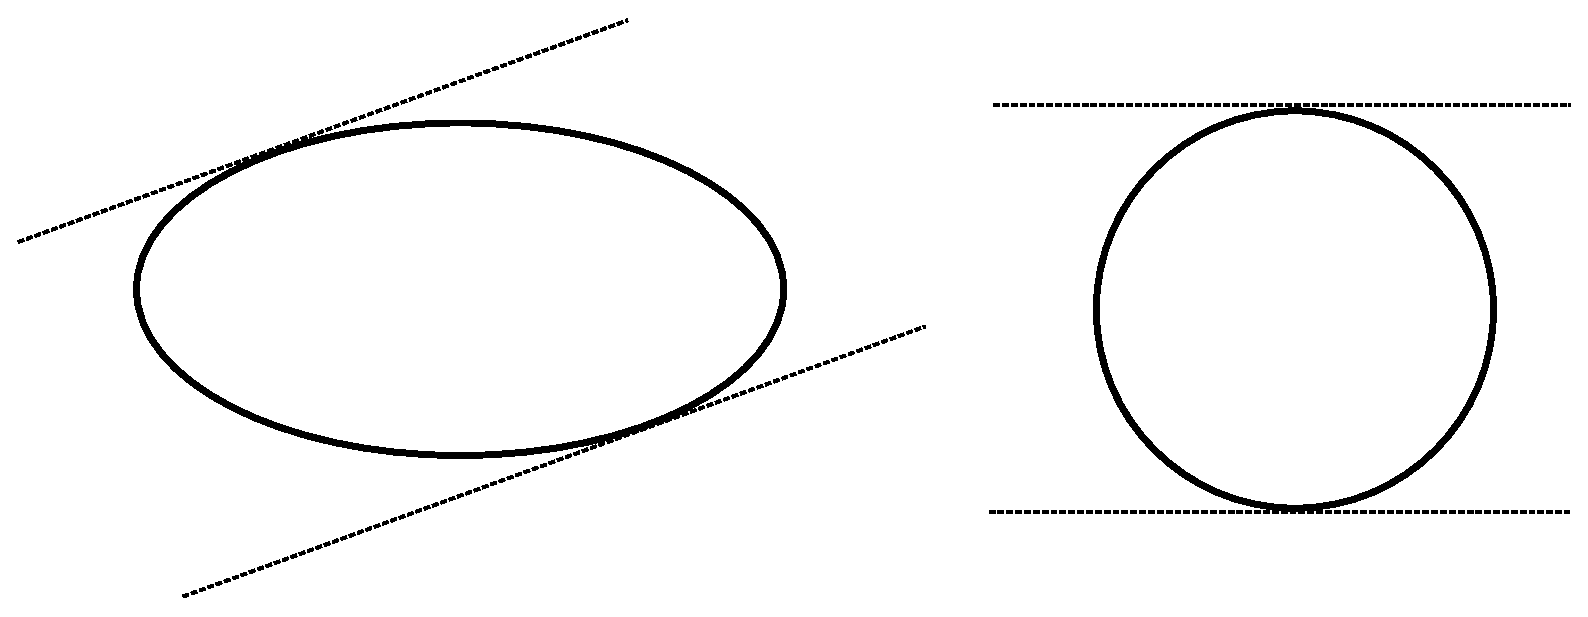
\includegraphics[width=0.5\columnwidth]{ellipse-new-ellipse}
      
      \caption{Отображение эллипса в окружность.}
      \label{fig:ellipse-new-ellipse}
    \end{figure}
    
    Рассмотрим сначала случай с эллипсом (\ref{fig:ellipse-new-ellipse}).
    Пусть две касательные к эллипсу параллельны.
    Обозначим точки касания за $A$ и $B$, а центр эллипса за $O$.
    Аффинным преобразованием переведём эллипс в окружность (для двух данных кривых второго порядка существует аффинное преобразование, которое переводит одну кривую в другую).
    При аффинном преобразовании прямая переходит в прямую, и параллельные прямые переходят в параллельные прямые.
    Поэтому образы параллельных касательных к эллипсу~---~параллельные касательные к окружности.
    Для окружности, очевидно, точки касания и центр будут лежать на одной прямой, точнее центр будет лежать не отрезке с концами в точках касания параллельных касательных.
    Обратным аффинным преобразованием переводим окружность обратно в эллипс.
    Отрезок при аффинном преобразовании переходит в отрезок, поэтому и в случае эллипса центр также будет лежать на отрезке с концами в касательных.
    
    Пусть точки касания эллипса лежат на одной прямой с центром эллипса.
    Аналогичным аффинным преобразованием можно перевести эллипс снова в окружность.
    При этом точки касания останутся на одной прямой с центром.
    Для окружности снова ``всё понятно''.
    Обратным преобразованием переводим окружность в эллипс, при этом параллельность прямых сохраняется.
    
    \bigskip

    \begin{figure}
      \centering
      
      \includegraphics[width=0.5\columnwidth]{hyperbola-new-hyperbola}  % TODO: нужны нормальные гиперболы)
      
      \caption{Отображение гиперболы в гиперболу.}
      \label{fig:hyperbola-new-hyperbola}
    \end{figure}

    Для гиперболы всё аналогично.
    Сохраним обозначения для точек касания и для центра.
    Пусть вначале касательные параллельны.
    Некоторым аффинным преобразованием исходную гиперболу можно перевести в такую гиперболу, чтоб образы параллельных касательных касались её в вершинах (\ref{fig:hyperbola-new-hyperbola})\footnote{Можно рассмотреть одну из ветвей гиперболы. Точку касания надо перевести в вершину ветви новой гиперболы. Пусть ось новой гиперболы~---~ось $X$. Можно взять ещё по одной точке ``слева'' и ``справа'' от точки касания, и потребовать, чтобы на новой гиперболе они бы располагались симметрично относительно оси $X$. Отображение трёх точек, не лежащих на одной прямой, задаёт аффинное преобразование. Гипербола при аффинном преобразовании переходит в гиперболу, отрезок в отрезок, параллельные прямые в параллельные прямые...}.
    Для такой гиперболы очевидно, что точки касания и центр лежат на одной прямой.
    Обратное преобразование, ...
    
    Пусть точки касания и центр лежат на одной прямой.
    Аффинным преобразованием переводим гиперболу снова в такую, чтоб точки касания перешли в вершины гиперболы-образа.
    Очевидно, касательные-образы параллельны.
    Обратное преобразование, ...
  \end{solution}
  
  
  \subsection{\# 12.26}
  
  Аффинное преобразование переводит три точки $A$, $B$, $C$, не лежащие на одной прямой, соответственно в точки $B$, $C$, $A$.
  Найти неподвижные точки этого преобразования.
  При каком необходимом и достаточном условии преобразование будет ортогональным\footnote{Ортогональное преобразование $f$~---~сохраняющее длины: $|AB| \hm= \bigr|f(A)f(B)\bigl|$. Так как вычисление длин в конечном итоге сводится к вычислению скалярных произведений между базисными векторами, то об ортогональном преобразовании можно думать и как о преобразовании, сохраняющем скалярные произведения.}?
  
  \begin{solution}
    Можно бы было решать задачу ``полностью'' координатным методом: ввести некоторую декартову систему координат на плоскости, через координаты точек $A$, $B$, и $C$ выразить коэффициенты аффинного преобразования и потом искать неподвижную точку как решение системы с, возможно, довольно громоздкими коэффициентами...
    
    Пойдём чуть более интеллектуальным путём.
    Три исходные точки не лежат на одной прямой.
    Значит, два из трёх векторов, которые можно построить на точках $A$, $B$ и $C$, можно взять в качестве базиса на плоскости.
    Зная образы базисных векторов, можно по ним разложить и любой вектор-образ\footnote{
      Образ вектора при аффинном преобразовании $f$ имеет в новом базисе те же координаты, что и исходный вектор в исходном базисе: $\bds v \hm= a \bds e_1 \hm+ b \bds e_2 \hm\Rightarrow f(\bds v) \hm= a f(\bds e_1) \hm+ b f(\bds e_2)$.
    }.
    Итак, предлагается выбрать векторы $\vv{AB} \hm\equiv \bds e_1$ и $\vv{BC} \hm\equiv \bds e_2$ в качестве базиса на плоскости.
    Образы базисных векторов:
    \[
      \left\{
        \begin{aligned}
          &\vv{AB} \mapsto \vv{BC}\\
          &\vv{BC} \mapsto \vv{CA}
        \end{aligned}
      \right.
    \]
    
    Обозначим образы базисных векторов за $\bds e_1'$ и $\bds e_2'$ и выразим их через исходные вектора
    \[
      \left\{
        \begin{aligned}
          &\bds e_1' = \vv{BC} = \bds e_2\\
          &\bds e_2' = \vv{CA} = \vv{CB} + \vv{BA} = -\bds e_2 - \bds e_1
        \end{aligned}
      \right.
    \]
    
    Мы хотим в итоге получить формулы для выражения координат $x'$, $y'$ точек через исходные координаты $x$, $y$.
    Для этого надо, наоборот, найти выражение \emph{исходных} базисных векторов через новые.
    Но это не сложно сделать:
    \[
      \left\{
        \begin{aligned}
          &\bds e_1 = -\bds e_1' - \bds e_2'\\
          &\bds e_2 = \bds e_1'
        \end{aligned}
      \right.
    \]
    
    Матрица перехода:
    \[
      S = \begin{pmatrix}-1 & 1\\ -1 & 0\end{pmatrix}
    \]
    
    Выражения для координат:
    \[
      \left\{
        \begin{aligned}
          &x^\star = -x + y + c_1\\
          &y^\star = -x + c_2
        \end{aligned}
      \right.
    \]
    
    \textbf{Но} перед тем, как писать выражения для координат, надо было выбрать начало системы координат (до этого были выбраны только базисные вектора).
    Для дальнейшего удобства решения предлагается выбрать начало не случайным, а равным, например, точке $A$.
    То есть полагаем $A(0, 0)$.
    
    Теперь можно выписать три системы из двух уравнений каждая для образов данных в условии задачи точек:
    \begin{equation}
      \label{eq:huge-system}
      \left\{
        \begin{aligned}
          &\left\{
            \begin{aligned}
              &x_A^\star = -x_A + y_A + c_1 = x_B\\
              &y_A^\star = -x_A + c_2 = y_B
            \end{aligned}
          \right.\\
          &\left\{
            \begin{aligned}
              &x_B^\star = -x_B + y_B + c_1 = x_C\\
              &y_B^\star = -x_B + c_2 = y_C
            \end{aligned}
          \right.\\
          &\left\{
            \begin{aligned}
              &x_C^\star = -x_C + y_C + c_1 = x_A\\
              &y_C^\star = -x_C + c_2 = y_A
            \end{aligned}
          \right.\\
        \end{aligned}
      \right.
    \end{equation}
    
    Из самой первой системы можно найти недостающие коэффициенты преобразования $c_1 \hm= x_B$ и $c_2 \hm= y_B$.
    Найдя эти коэффициенты, неподвижную точку можно найти как решение системы:
    \[
      \left\{
        \begin{aligned}
          &x = -x + y + c_1\\
          &y = -x + c_2
        \end{aligned}
      \right.
      \Leftrightarrow
      \left\{
        \begin{aligned}
          &x = \frac{c_1 + c_2}{3}\\
          &y = \frac{-c_1 + 2c_2}{3}
        \end{aligned}
      \right.
    \]
    
    То есть неподвижная точка получилась равной $\left(\dfrac{x_B + y_B}{3}, \dfrac{-x_B + 2y_B}{3}\right)$. На этом можно бы было, наверно, считать задачу решённой... но хоть ответ есть, он получился ``непонятный''.
    Чтобы ответ можно было ``потрогать'', надо получить выражения $x$ и $y$ компонент неподвижной точки через $x$ и $y$ компоненты точек из условия соответственно.
    Для этого надо вернуться к системе (\ref{eq:huge-system}) и выразить $c_1$ и $c_2$ по-другому.
    Можно бы было, наверное, сделать замену $c_1 \hm+ c_2$ и $-c_1 \hm+ 2c_2$~---~тогда бы было понятнее, что хочется получить при решении системы.
    Но можно и так (никаких подстановок делать не потребуется: надо просто выразить $c_1$ и $c_2$ из каждой из трёх систем и потом с этим ``играть'').
    В итоге координаты неподвижной точки:
    \[
      \left\{
        \begin{aligned}
          &x = \frac{(x_C + x_B - y_B) + (y_B)}{3} = \frac{x_B + x_C}{3}\\
          &y = \frac{-(y_B - y_C) + 2(y_B)}{3} = \frac{y_B + y_C}{3}
        \end{aligned}
      \right.
    \]
    
    Теперь понятно, что эта точка~---~точка пересечения медиан треугольника $ABC$!
    
    \bigskip
    
    Второй вопрос задачи кажется намного проще первого.
    Преобразование ортогональное, если оно сохраняет длины.
    Поэтому надо потребовать, чтобы длины образов базисных векторов были такими же, как и длины исходных векторов, и чтобы угол между образами был такой же, как и угол между прообразами.
    Условие на длины:
    \[
      \left\{
        \begin{aligned}
          &AB = BC\\
          &BC = CA
        \end{aligned}
      \right.
    \]
    означает, что треугольник $ABC$ равносторонний.
    При этом угол между образами базисных векторов тоже не меняется (остаётся равным $120\degree$).
  \end{solution}
  
  
  \subsection{Ещё задача}
  
  Для аффинного преобразования плоскости
  \[
    \left\{
      \begin{aligned}
        &x^\star = 6x - y + 2\\
        &y^\star = 7x - 3y + 4
      \end{aligned}
    \right.
  \]
  надо найти
  \begin{enumerate}
    \item Площадь образа круга радиуса $1$
    \item Площадь прообраза круга радиуса $1$
    \item Все неподвижные точки
    \item Все инвариантные прямые
  \end{enumerate}
  
  \begin{solution}
    Рассмотрим два неколлинеарных вектора $\bds u$ и $\bds v$.
    Площадь параллелограмма, построенного на этих векторах:
    \[
      S_{\pm}(\bds u, \bds v) = \begin{vmatrix}u_1 & u_2\\ v_1 & v_2\end{vmatrix} \cdot S_{\pm}(\bds e_1, \bds e_2)
    \]
    
    При аффинном преобразовании $f$ компоненты образов векторов в новом базисе получаются такими же, как в старом.
    Поэтому для площади параллелограмма, построенного на векторах $\bds u^\star$ и $\bds v^\star$ верно
    \[
      S_{\pm}(\bds u^\star, \bds v^\star) = \begin{vmatrix}u_1 & u_2\\ v_1 & v_2\end{vmatrix} \cdot S_{\pm}\bigl(\bds e_1^\star, \bds e_2^\star\bigr)
      = \begin{vmatrix}u_1 & u_2\\ v_1 & v_2\end{vmatrix} \begin{vmatrix}a_1 & a_2\\ b_1 & b_2\end{vmatrix} \cdot S_{\pm}(\bds e_1, \bds e_2)
    \]
    где в последнем переходе образы базисных векторов были выражены в исходном базисе.

    Откуда отношение площади после преобразования к площади до преобразования:
    \[
      \frac{S^\star}{S} = \begin{vmatrix}a_1 & a_2\\ b_1 & b_2\end{vmatrix} = \begin{vmatrix}a_1 & b_1\\ a_2 & b_2\end{vmatrix}
    \]
    
    Возвращаясь к задаче, отношение площадей по модулю будет равным
    \[
      \left|\det\begin{pmatrix}
        6 & -1\\
        7 & -3
      \end{pmatrix}\right| = 11
    \]
    
    Поэтому площадь образа круга радиуса $1$ будет равна $11 \pi\ \mbox{ед}^2$.
    
    Обратно, площадь прообраза круга радиуса $1$ будет равна $\dfrac{\pi}{11}\ \mbox{ед}^2$.
    
    Чтобы найти неподвижные точки преобразования, надо решить систему
    \[
      \left\{
        \begin{aligned}
          &x = 6x - y + 2\\
          &y = 7x - 3y + 4
        \end{aligned}
      \right.
      \Rightarrow \ldots
      \Rightarrow \left\{
        \begin{aligned}
          &x = -\frac{4}{13}\\
          &y = \frac{6}{13}
        \end{aligned}
      \right.
    \]
    
    Инвариантные прямые можно искать в виде $Ax + By + C \hm= 0$.
    Прямая $l$ инварианта относительно преобразования $f$, если $M \hm\in l \hm\Rightarrow M^\star \hm= f(M) \hm\in l$.
    То есть
    \begin{equation*}
    \begin{split}
      \left\{
        \begin{aligned}
          &Ax + By + C = 0\\
          &Ax^\star + By^\star + C = 0
        \end{aligned}
      \right.
      &\Leftrightarrow \left\{
        \begin{aligned}
          &Ax + By + C = 0\\
          &A \cdot (6x - y + 2) + B \cdot (7x - 3y + 4) + C = 0
        \end{aligned}
      \right.\\
      &\Leftrightarrow \left\{
        \begin{aligned}
          &Ax + By + C = 0\\
          &(6A + 7B) x + (-A - 3B) y + (2A + 4B + C) = 0
        \end{aligned}
      \right.
    \end{split}
    \end{equation*}
    
    Получаем условие на коэффициенты преобразования
    \[
      \frac{6A + 7B}{A} = \frac{-A - 3B}{B} = \frac{2A + 4B + C}{C}
    \]
    
    Решая получившуюся систему, и учитывая, что $A^2 \hm+ B^2 \hm> 0$, находим коэффициенты в уравнении прямых
    \[
      \left\{
        \begin{aligned}
          &A = B \cdot \left(-\frac{9}{2} \pm \frac{\sqrt{53}}{2}\right)\\
          &C = B \cdot \left(-\frac{24}{13} \pm \frac{2\sqrt{53}}{13}\right)
        \end{aligned}
      \right.
    \]
    
    И уравнения инвариантных прямых (при $B \hm= 26$):
    \[
      13\left(-9 \pm \sqrt{53}\right)x + 26y + 2\left(-24 \pm 2\sqrt{53}\right) = 0
    \]
  \end{solution}
  
  % TODO: задача про разложение в сжатия и ортогональное
\end{document}
